\documentclass[12pt,a4paper]{article}
\usepackage[margin=2.5cm]{geometry}
\usepackage{amsmath,amssymb}
\usepackage{booktabs}
\usepackage{array}
\usepackage{xcolor}
\usepackage{listings}
\usepackage{hyperref}
\usepackage{tikz}
\usetikzlibrary{positioning,arrows.meta,shapes.geometric}
\usepackage{multirow}
\usepackage{caption}
\usepackage{float}

\hypersetup{colorlinks=true, linkcolor=blue, urlcolor=blue}

\lstset{
  basicstyle=\ttfamily\small,
  backgroundcolor=\color{gray!10},
  frame=single,
  breaklines=true,
  keywordstyle=\color{blue},
  commentstyle=\color{gray},
}

\title{\textbf{SKALD Pipeline: New Innovations}\\[0.5em]
\large Non-Uniform Interval Hierarchies, Two-Pass Architecture, \\ and Parameter Grid}
\author{}
\date{}

\begin{document}
\maketitle
\tableofcontents
\newpage

% =============================================================================
\section{Overview}

This document describes innovations added to the SKALD k-anonymisation pipeline,
assuming the reader is familiar with the baseline system (OLA-1/OLA-2 lattice
search, sparse histogram, DM* scoring).

The three major additions are:
\begin{enumerate}
  \item \textbf{Non-uniform interval hierarchies with configurable split factor} — user-defined
        coarse intervals are automatically refined into a multi-level hierarchy by
        repeatedly splitting each interval into $n$ equal parts (halving when $n{=}2$,
        decile split when $n{=}10$, etc.), replacing the fixed uniform bin-width model
        for numerical quasi-identifiers (QIs).  The split factor $n$ is taken from
        the existing \texttt{size} config field for the column.
  \item \textbf{Two-pass architecture} — a \texttt{pass1} run computes the
        optimal $k$ recommendation and a preview grid; a separate \texttt{pass2}
        run executes full anonymisation with the user-chosen $k$.
  \item \textbf{Parameter grid} — a sparse $(k \times \text{suppression\_limit})$
        table giving the best generalization node, DM* score, equivalence-class
        count, and suppression count for each combination.
\end{enumerate}

% =============================================================================
\section{Non-Uniform Interval Hierarchies}

\subsection{Motivation}

The original pipeline generalised numerical QIs with a uniform step size
(bin width). This is adequate when values are uniformly spread, but poor when
domain knowledge suggests natural groupings — e.g.\ age brackets by life stage
or PIN codes by postal region.

The new system lets users define \emph{arbitrary coarse intervals} for any
numerical QI. The pipeline then automatically constructs a full multi-level
hierarchy by repeatedly halving those intervals, down to single-value bins.

\subsection{User Configuration}

Intervals are declared in the JSON config under \texttt{qi\_constraints}:

\begin{lstlisting}[language={}]
"qi_constraints": {
  "Age": {
    "intervals": [
      {"from": 22, "to": 30},
      {"from": 31, "to": 45},
      {"from": 46, "to": 60},
      {"from": 61, "to": 75}
    ]
  },
  "PIN Code": {
    "intervals": [
      {"from": 110000, "to": 300000},
      {"from": 300001, "to": 500000},
      {"from": 500001, "to": 700000},
      {"from": 700001, "to": 797001}
    ]
  }
}
\end{lstlisting}

Multiple QIs can each have their own independent interval constraints.
QIs without a \texttt{qi\_constraints} entry continue to use uniform bin-width
generalization as before.

\subsection{Hierarchy Construction}

\subsubsection{Split Factor}

Each QI with interval constraints has an associated \textbf{split factor} $n$,
taken from the \texttt{size} config field for that column (default $n{=}2$).
The split factor controls how many sub-intervals each interval is divided into
at every refinement step.

\begin{lstlisting}[language={}]
"size": { "Age": 2, "PIN Code": 10 }
\end{lstlisting}

Age uses $n{=}2$ (binary halving); PIN Code uses $n{=}10$ (decile split).

\subsubsection{Number of Levels}

Given the minimum bin width $w_{\min}$ of the user's coarse intervals and the
split factor $n$, the number of refinement steps is the largest integer $s$
such that repeatedly dividing by $n$ keeps the minimum width $\geq n$:

\begin{equation}
  w_{\min} = \min_{i}\bigl(to_i - from_i + 1\bigr)
\end{equation}

\begin{equation}
  \text{num\_splits} = \begin{cases}
    0 & \text{if } w_{\min} < n \\
    \lfloor \log_n(w_{\min}) \rfloor & \text{otherwise}
  \end{cases}
\end{equation}

\begin{equation}
  \boxed{L = 1 + \text{num\_splits}}
\end{equation}

Splitting stops when the minimum interval width would drop below $n$ (i.e.\
it is no longer meaningful to split into $n$ parts).

\subsubsection{General Split Rule}

Each interval $[from, to]$ with width $w = to - from + 1$ is split into
$n$ sub-intervals:

\begin{align}
  p &= \lfloor w / n \rfloor \quad\text{(part size)} \\
  \text{Sub-interval } i &=
    \begin{cases}
      [from + i \cdot p,\; from + (i+1) \cdot p - 1] & i < n-1 \\
      [from + (n-1) \cdot p,\; to]                    & i = n-1 \text{ (absorbs remainder)}
    \end{cases}
\end{align}

Intervals with width $< n$ are left unchanged (cannot be meaningfully divided).

\subsubsection{Worked Example — Age ($n=2$, halving)}

User intervals: $[22\text{--}30],\ [31\text{--}45],\ [46\text{--}60],\ [61\text{--}75]$.

\begin{align*}
  w_{\min} &= 9 \qquad (\text{width of }[22\text{--}30]) \\
  \text{num\_splits} &= \lfloor\log_2(9)\rfloor = 3 \\
  L &= 4
\end{align*}

\begin{table}[H]
\centering
\caption{Age Interval Hierarchy ($n{=}2$, 4 levels)}
\begin{tabular}{ccp{9cm}}
\toprule
Level & \#Intervals & Intervals \\
\midrule
4 (coarsest) & 4 & $[22\text{--}30]\ [31\text{--}45]\ [46\text{--}60]\ [61\text{--}75]$ \\
3 & 8 & $[22\text{--}26]\ [27\text{--}30]\ [31\text{--}38]\ [39\text{--}45]\ [46\text{--}53]\ [54\text{--}60]\ [61\text{--}68]\ [69\text{--}75]$ \\
2 & 16 & $[22\text{--}24]\ [25\text{--}26]\ [27\text{--}28]\ [29\text{--}30]\ \ldots$ \\
1 (finest) & 32 & $[22\text{--}23]\ [24\text{--}24]\ [25\text{--}25]\ \ldots$ \\
\bottomrule
\end{tabular}
\end{table}

\subsubsection{Worked Example — PIN Code ($n=10$, decile split)}

User intervals: $[110000\text{--}300000],\ [300001\text{--}500000],\
[500001\text{--}700000],\ [700001\text{--}797001]$.

\begin{align*}
  w_{\min} &= 797001 - 700001 + 1 = 97001 \\
  \text{num\_splits} &= \lfloor\log_{10}(97001)\rfloor = \lfloor 4.987 \rfloor = 4 \\
  L &= 5
\end{align*}

\begin{table}[H]
\centering
\caption{PIN Code Interval Hierarchy ($n{=}10$, 5 levels)}
\begin{tabular}{ccp{9cm}}
\toprule
Level & \#Intervals & Description \\
\midrule
5 (coarsest) & 4 & User-defined postal regions \\
4 & 40 & Each region split into 10 sub-regions \\
3 & 400 & Each split again into 10 \\
2 & 4\,000 & Min width $\approx 97$ \\
1 (finest) & 40\,000 & Min width $\approx 9$--$10$ \\
\bottomrule
\end{tabular}
\end{table}

For example, $[700001\text{--}797001]$ with $w{=}97001$, $p{=}9700$:
\[
  [700001\text{--}709700]\ [709701\text{--}719400]\ \cdots\ [787301\text{--}797001]
\]

\paragraph{Comparison with halving.}
With $n{=}2$ (the old behaviour) PIN Code would require
$\lfloor\log_2(97001)\rfloor = 16$ halvings, producing $4 \times 2^{16} = 262\,144$
fine intervals. With $n{=}10$ only $4 \times 10^4 = 40\,000$ fine intervals are
needed across 5 levels instead of 17 — a $6.6\times$ reduction in lattice depth
and an $85\%$ reduction in the finest-level interval count, dramatically lowering
memory and search cost.

\subsubsection{Ancestor Lookup Table}

For fast generalization during histogram merging and output writing, the
system precomputes for every fine interval $f$ (at level 1) its ancestor
index at every coarser level:

\[
  \texttt{ancestor\_at}[f][\ell] = \text{index of the level-}\ell
  \text{ interval that contains fine interval }f
\]

Lookup uses binary search ($O(\log n)$ per call) since intervals at every
level are stored in sorted order by their left endpoint.

\subsection{Lattice Representation of Interval QIs}

In the original OLA lattice, a numerical QI node coordinate is a bin width
(e.g.\ 5, 10, $\ldots$, range). For interval QIs the coordinate is instead
the \emph{level number}, ranging from 1 (finest) to $L$ (coarsest):

\begin{center}
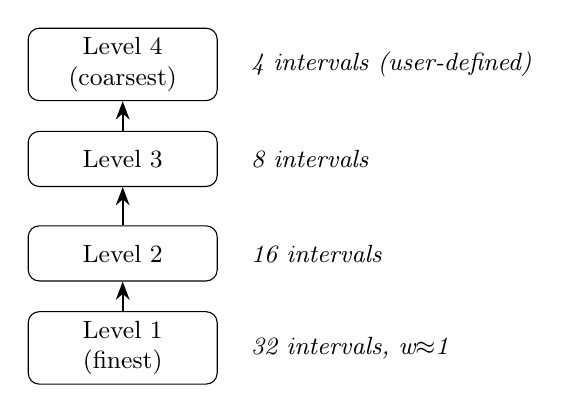
\begin{tikzpicture}[
  node distance=1.2cm,
  box/.style={draw, rounded corners, minimum width=2.4cm, minimum height=0.7cm,
              font=\small, align=center},
  arr/.style={-{Stealth}, thick}
]
\node[box] (l1) {Level 1\\(finest)};
\node[box, above of=l1] (l2) {Level 2};
\node[box, above of=l2] (l3) {Level 3};
\node[box, above of=l3] (l4) {Level 4\\(coarsest)};
\draw[arr] (l1) -- (l2);
\draw[arr] (l2) -- (l3);
\draw[arr] (l3) -- (l4);
\node[right=0.3cm of l1, font=\small\itshape] {32 intervals, w$\approx$1};
\node[right=0.3cm of l2, font=\small\itshape] {16 intervals};
\node[right=0.3cm of l3, font=\small\itshape] {8 intervals};
\node[right=0.3cm of l4, font=\small\itshape] {4 intervals (user-defined)};
\end{tikzpicture}
\end{center}

Stepping \emph{up} the lattice (toward coarser generalization) increments the
level coordinate by 1, instead of multiplying a bin width by a factor.

\subsection{Multi-QI Lattice with Mixed Types}

When multiple QIs are used together — some with interval constraints, some
uniform numerical, some categorical — the lattice node is a vector:

\[
  \mathbf{n} = (\ell_{\text{Age}},\ \ell_{\text{PIN}},\ \ell_{\text{Blood}})
\]

\begin{table}[H]
\centering
\caption{Node coordinate semantics by QI type}
\begin{tabular}{llll}
\toprule
QI & Type & Split factor & Coordinate meaning \\
\midrule
Age      & Interval hierarchy ($L{=}4$) & $n{=}2$ & Level $\in \{1,2,3,4\}$ \\
PIN Code & Interval hierarchy ($L{=}5$) & $n{=}10$ & Level $\in \{1,\ldots,5\}$ \\
Blood Group & Categorical (3 levels)   & —        & Level $\in \{1,2,3\}$ \\
\bottomrule
\end{tabular}
\end{table}

The bottom of the lattice (most specific) is $(1,1,1)$; the top (most general)
is $(4,5,3)$. The lattice has $4 \times 5 \times 3 = 60$ distinct nodes
(compared to $4 \times 17 \times 3 = 204$ with halving for PIN Code).

OLA-2 binary-searches this lattice exactly as before; the only change is how
each coordinate is interpreted when merging the histogram.

% =============================================================================
\section{Two-Pass Architecture}

\subsection{Motivation}

$k$ is a user-facing privacy parameter. Choosing it blindly is difficult:
too low gives little protection; too high suppresses too many records or
forces coarse generalization. The two-pass design separates
\emph{exploration} (what $k$ is feasible?) from \emph{execution} (apply the
chosen $k$ and produce output).

\subsection{Pass Trigger in Config}

A single field in the JSON config selects the pipeline mode:

\begin{lstlisting}[language={}]
"pass": "pass1"      // explore only — no output CSV produced
"pass": "pass2"      // full run with preprocessing and k set by user
"pass": "no_bounds"  // legacy single-pass, no interval constraints needed
\end{lstlisting}

\subsection{Pass 1: Exploration}

\textbf{What runs:} chunking $\to$ min/max scan $\to$ QI building $\to$
OLA-1 $\to$ sparse histogram $\to$ parameter grid $\to$ $k_{\text{opt}}$ computation.

\textbf{What does NOT run:} preprocessing (suppress, hash, encrypt, etc.) and
OLA-2/generalization (no output CSV is written).

\textbf{Output} (in \texttt{output/status.json}, phase \texttt{awaiting\_pass2}):

\begin{lstlisting}[language={}]
{
  "pass": "pass1",
  "k_optimal": 489,
  "total_records": 50000,
  "suppression_limit": 0.05,
  "parameter_grid": [ ... ],
  "histogram_buckets": 5554,
  "initial_ri": [1, 1, 1]
}
\end{lstlisting}

The user reads \texttt{parameter\_grid.txt} (human-readable table) and
\texttt{status.json}, chooses a $(k, \text{suppression\_limit})$ combination,
then sets those values in \texttt{config\_pass2.json} before triggering pass 2.

\subsection{Optimal \texorpdfstring{$k$}{k} Recommendation (\texorpdfstring{$k_{\text{opt}}$}{k\_opt})}

$k_{\text{opt}}$ is computed at the \emph{coarsest constrained node} — the
node where each interval QI is at its user-defined coarse level, each
categorical QI is at its maximum level, and each uniform numerical QI collapses
to a single bin.

Let $\mathcal{E}_c$ be the multiset of equivalence-class sizes at the coarsest
node. Sort them in ascending order:
$s_1 \leq s_2 \leq \cdots \leq s_m$.

The allowed suppression budget is:
\[
  B = \lfloor \sigma \cdot N \rfloor
  \qquad \text{where } \sigma = \text{suppression\_limit},\ N = \text{total records}
\]

Walk the sorted sizes, accumulating a running prefix $P$:

\begin{equation}
  k_{\text{opt}} = \max\bigl\{s_j \mid P_{j-1} \leq B\bigr\}
  \qquad\text{where }P_j = \sum_{i=1}^{j} s_i
\end{equation}

Intuitively: $k_{\text{opt}}$ is the largest equivalence-class size such that
all classes \emph{smaller} than it (which would be suppressed if $k =
k_{\text{opt}}$) together fit within the suppression budget.

\paragraph{Example.} Classes: $[1, 2, 3, 50, 50, 50, 50]$, $B = 10$.

\begin{table}[H]
\centering
\begin{tabular}{rrrrl}
\toprule
$j$ & $s_j$ & $P_{j-1}$ & $P_{j-1} \leq B$? & $k_{\text{opt}}$ candidate \\
\midrule
1 & 1  & 0  & yes & 1 \\
2 & 2  & 1  & yes & 2 \\
3 & 3  & 3  & yes & 3 \\
4 & 50 & 6  & yes & \textbf{50} \\
5 & 50 & 56 & no  & — \\
\bottomrule
\end{tabular}
\end{table}

Result: $k_{\text{opt}} = 50$ (not 3 or 1 — the suppression budget permits
discarding the three small classes).

\subsection{Pass 2: Full Anonymisation}

\textbf{What runs:} chunking $\to$ preprocessing $\to$ min/max $\to$ QIs $\to$
OLA-1 $\to$ histogram $\to$ parameter grid $\to$ OLA-2 $\to$
generalization $\to$ output CSV.

Config must include \texttt{"k\_anonymize": \{"k": <chosen\_value>\}}.
Preprocessing fields (suppress, hash, encrypt, etc.) are active.
The output CSV is the fully anonymised dataset.

% =============================================================================
\section{Parameter Grid}

\subsection{Purpose}

After the histogram is built (in \emph{both} passes), the pipeline runs
OLA-2 for a sparse grid of $(k, \sigma)$ pairs and records the best
generalization node, DM* score, equivalence-class count, and suppression count
for each combination. This gives the user a concise view of the
privacy--utility trade-off before committing to a choice.

\subsection{Grid Values}

\[
  k \in \{5,\ 10,\ 50,\ 100\}
  \qquad
  \sigma \in \{0.00,\ 0.01,\ 0.10\}
\]

Twelve cells in total. Each cell executes a full OLA-2 binary search on the
already-built in-memory histogram, so the added cost is negligible.

\subsection{Grid Entry Fields}

\begin{table}[H]
\centering
\caption{Fields in each parameter grid entry}
\begin{tabular}{ll}
\toprule
Field & Meaning \\
\midrule
\texttt{k} & Privacy threshold \\
\texttt{suppression\_limit} ($\sigma$) & Fraction of records allowed to be suppressed \\
\texttt{best\_node} & Lattice node (level vector) with lowest DM* \\
\texttt{dm\_star} & Discernibility metric at the best node \\
\texttt{num\_equivalence\_classes} & Number of equivalence classes at best node \\
\texttt{suppression\_count} & Records suppressed at best node \\
\texttt{feasible} & Whether any k-anonymous node exists \\
\bottomrule
\end{tabular}
\end{table}

\subsection{Output Files}

Two files are written every run:

\begin{itemize}
  \item \texttt{output/status.json} — full JSON including the grid under
        \texttt{outputs.parameter\_grid}.
  \item \texttt{output/parameter\_grid.txt} — human-readable table for quick
        inspection.
\end{itemize}

\subsection{Sample Table (50\,000-record test dataset)}

\begin{table}[H]
\centering
\caption{Parameter grid — Age + PIN Code + Blood Group QIs}
\begin{tabular}{rrllrrrl}
\toprule
$k$ & $\sigma$ & Best node & DM* & ECs & Suppressed & Feasible \\
\midrule
5   & 0.00 & [1, 17, 3] &  9\,612\,310 &  384 &     0 & yes \\
5   & 0.01 & [2,  1, 3] &  3\,531\,723 & 1098 &   369 & yes \\
5   & 0.10 & [1,  2, 1] &  1\,357\,413 & 2614 & 3\,847 & yes \\
10  & 0.00 & [2, 17, 2] & 15\,383\,904 &  256 &     0 & yes \\
10  & 0.01 & [3,  1, 3] &  6\,900\,405 &  550 &   419 & yes \\
10  & 0.10 & [1,  1, 3] &  1\,824\,713 & 1562 & 3\,515 & yes \\
50  & 0.00 & [3, 17, 3] & 36\,518\,880 &   96 &     0 & yes \\
50  & 0.01 & [2, 17, 3] & 18\,581\,303 &  186 &   237 & yes \\
50  & 0.10 & [1, 16, 3] &  6\,567\,006 &  374 & 4\,842 & yes \\
100 & 0.00 & [4, 17, 3] & 72\,448\,990 &   48 &     0 & yes \\
100 & 0.01 & [3, 17, 3] & 36\,496\,690 &   93 &   258 & yes \\
100 & 0.10 & [2, 16, 3] & 12\,707\,298 &  194 & 4\,376 & yes \\
\bottomrule
\end{tabular}
\end{table}

Node coordinates are $(\ell_{\text{Age}},\ \ell_{\text{PIN}},\
\ell_{\text{Blood}})$ where Age has 4 levels, PIN Code has 17 levels,
and Blood Group has 3 levels.

\paragraph{Reading the table.}
Moving left-to-right in each row, higher $k$ demands coarser generalization
(larger DM*, fewer ECs). Within a fixed $k$, allowing more suppression
($\sigma$ increasing) enables finer generalization (lower DM*, more ECs),
because small equivalence classes that cannot reach $k$ are dropped rather
than merged with neighbours.

% =============================================================================
\section{RAM-Adaptive Chunking}

The original pipeline used a hardcoded 50\,000 rows per chunk. The new
system targets 20\% of available RAM per chunk:

\begin{equation}
  \text{rows\_per\_chunk} =
  \left\lfloor \frac{0.20 \times \text{MemAvailable}}{b_{\text{row}}} \right\rfloor
\end{equation}

where $b_{\text{row}}$ is the average byte length of a data row, estimated by
sampling the first 200 rows of the CSV. The result is clamped to
$[1\,000,\ 10\,000\,000]$.

Available RAM is read from \texttt{/proc/meminfo} (\texttt{MemAvailable}),
making the pipeline safe to run on both small containers and large servers
without manual tuning.

% =============================================================================
\section{Summary of Changes to the Lattice}

\begin{table}[H]
\centering
\caption{Lattice coordinate semantics: before and after}
\begin{tabular}{lll}
\toprule
QI type & Before & After \\
\midrule
Uniform numerical & Bin width (1, factor, $\ldots$, range) & Unchanged \\
Categorical & Level (1, 2, 3) & Unchanged \\
Interval-constrained numerical & Not supported &
  Level 1 (finest) $\to$ $L$ (coarsest); $L = 1 + \lfloor\log_n(w_{\min})\rfloor$ \\
\bottomrule
\end{tabular}
\end{table}

The split factor $n$ is read from the \texttt{size} config field for the column.
Setting $n{=}2$ reproduces binary halving; $n{=}10$ gives decile splits, which
is the recommended value for large-range columns such as PIN codes.

The OLA-1 and OLA-2 algorithms are unchanged algorithmically; only the
\emph{interpretation} of node coordinates and the \emph{histogram key
computation} differ for interval QIs. Histogram keys for interval QIs use the
fine-interval index (found via binary search) rather than a divided integer
value.

\end{document}
